\documentclass{article}
\usepackage{indentfirst}
\usepackage[utf8]{inputenc}
\usepackage[T1]{fontenc}
\usepackage[brazilian]{babel}
\usepackage{lmodern}
\usepackage{graphicx}
\usepackage{float}
\usepackage[]{subfigure}
\usepackage{afterpage}
\usepackage{amsmath}
\usepackage{textcomp,gensymb}
\usepackage{nameref}
\usepackage{accents}
\usepackage{listings}
\usepackage{color,soul}
\usepackage[margin=1in]{geometry}
\usepackage{steinmetz}

\PassOptionsToPackage{hyphens}{url}\usepackage{hyperref}
\hypersetup{
    breaklinks = true,
}
\urlstyle{same}
\newcommand{\ubar}[1]{\underaccent{\bar}{#1}}
\renewcommand\thesection{\arabic{section}$^a$}
\renewcommand\thesubsection{(\alph{subsection})}
\definecolor{dkgreen}{rgb}{0,0.6,0}
\definecolor{gray}{rgb}{0.5,0.5,0.5}
\definecolor{mauve}{rgb}{0.58,0,0.82}
\lstset{
    frame=tb,
    language=Matlab,
    aboveskip=3mm,
    belowskip=3mm,
    showstringspaces=false,
    basicstyle={\small\ttfamily},
    numbers=none,
    numberstyle=\tiny\color{gray},
    keywordstyle=\color{blue},
    commentstyle=\color{dkgreen},
    stringstyle=\color{mauve},
    breaklines=true,
    breakatwhitespace=true,
    tabsize=4
}

\title{Trabalho}
\author{Arthur Matos}
\date{2021}

\begin{document}
% capa
\begin{titlepage}
    \begin{center}
        \centering
        
\includegraphics[width=.7\linewidth]{images/logo_unb.png}\\[0.5cm]
        {\large \textbf{Universidade de Brasília}}\\[0.2cm]
        {\large \textbf{Departamento de Engenharia Elétrica}}\\[0.2cm]
        {\large \textbf{Controle Digital}}\\[4.8cm]
        {\bf \huge {Exercício de Simulação 2}}\\[0.2cm]
        {\bf \large {}}
    \end{center}

    \vspace{5cm}
    \hspace{2cm} {\noindent \bf \large {Aluno:}}\\
    \vspace{0.8cm}
    \hspace{2.35cm} {\large Arthur de Matos Beggs --------------------------------- 12/0111098}\\[1cm]

    \begin{center}
        {\large Brasília}\\
        {\large 2$^{\ubar{\circ}}$/2020}
    \end{center}

\end{titlepage}
\clearpage
\setcounter{page}{2}
% \tableofcontents
\clearpage

% % Template de figura
% \begin{figure}[H]
%     \centering
%         \includegraphics[width=1\linewidth]{images/}
%         \caption{}\label{fig:}
% \end{figure}

% % Corpo do Relatório

\section*{Discretize a função de transferência $$ G(s) = \frac{Y(s)}{U(s)} = \frac{1}{(s+2)(s+3)} $$ usando os métodos a seguir.}
\section*{Para cada caso, calcule a solução para $u(t) = 0$ $\forall\, t \geq 0$, $y(0) = 100$, $\dot{y}(0) = 0$, $T = 0.1s$ e compare no Matlab a solução exata a tempo contínuo com os resultados obtidos.}

\section{Transformada de $ G(s) $ com segurador de ordem zero em série:}
    \[ G(z) = (1-z^{-1}) \mathcal{Z}\left[ \frac{G(s)}{s} \right] = (1-z^{-1}) \mathcal{Z}\left[ \frac{1}{s(s+2)(s+5)} \right] \]
    {Expandindo em frações parciais:}
    \[ G(z) = (1-z^{-1}) \mathcal{Z}\left[ \frac{1}{6s} + \frac{1}{3(s+3)} + \frac{1}{2(s+2)} \right] = \left( \frac{z-1}{z} \right) \left( \frac 1 6 \frac{z}{z-1} + \frac 1 3 \frac{z}{z-e^{-3T}} - \frac 1 2 \frac{z}{z-e^{-2T}} \right) \]
    \[ G(z) = \frac{ 0.0042z + 0.0035 }{ z^2 - 1.5595z + 0.6065 } \]
    {Equação de diferenças:}
    \[ y[k](z^2 - 1.5595z + 0.6065) = u[k](0.0042z + 0.0035), u[k] = 0 \,\forall k \geq 0 \implies y[k](z^2 - 1.5595z + 0.6065) = 0 \]
    \[ y[k] = 1.5595 y[k-1] - 0.6065 y[k-2] \]
    \[ \begin{cases}
        y[0] = 100\\
        y[1] - y[2] = 0 \implies y[1] = y[2]
    \end{cases}\]


\section{Regra retangular para frente:}
    \[ G(z) = \left.G(s)\right|_{s=\frac{z-1}{T}}; T = 0.1 \]
    \[ G(z) = \frac{1}{\left( \left( \frac{z-1}{0.1}\right) +2 \right)\left( \left( \frac{z-1}{0.1}\right) +3 \right)} = \frac{0.001}{z^2 - 1.5z + 0.56} \]
    {Equação de diferenças:}
    \[ y[k](z^2 - 1.5z + 0.56) = 0.01 u[k], u[k] = 0 \,\forall k \geq 0 \implies y[k](z^2 - 1.5z + 0.56) = 0 \]
    \[ y[k] = 1.5 y[k-1] - 0.56 y[k-2] \]
    \[ \begin{cases}
        y[0] = 100\\
        y[1] - y[2] = 0 \implies y[1] = y[2]
    \end{cases}\]


\section{Regra retangular para trás:}
    \[ G(z) = \left.G(s)\right|_{s=\frac{z-1}{Tz}}; T = 0.1 \]
    \[ G(z) = \frac{1}{\left( \left( \frac{z-1}{0.1z} \right) +2 \right)\left( \left( \frac{z-1}{0.1z} \right) +3 \right)} = \frac{0.0064 z^2}{z^2 - 1.6025z + 0.641} \]
    {Equação de diferenças:}
    \[ y[k](z^2 - 1.6025z + 0.641) = 0.0064 z^2 u[k], u[k] = 0 \,\forall k \geq 0 \implies y[k](z^2 - 1.6025z + 0.641) = 0 \]
    \[ y[k] = 1.6025 y[k-1] - 0.641 y[k-2] \]
    \[ \begin{cases}
        y[0] = 100\\
        y[1] - y[2] = 0 \implies y[1] = y[2]
    \end{cases}\]


\section{Regra trapeizodal:}
    \[ G(z) = \left.G(s)\right|_{s=\frac 2 T\frac{z-1}{z+1}}; T = 0.1 \]
    \[ G(z) = \frac{1}{\left( \left( \frac{2}{0.1}\frac{z-1}{z+1} \right) +2 \right)\left(\left( \frac{2}{0.1}\frac{z-1}{z+1}\right) +3 \right)} = \frac{z^2 + 2z +1}{506z^2 - 788z + 306} \]
    {Equação de diferenças:}
    \[ y[k](506z^2 - 788z + 306) = z^2 + 2z + 1 u[k], u[k] = 0 \,\forall k \geq 0 \implies y[k](506z^2 - 788z + 306) = 0 \]
    \[ y[k] = \frac{788 y[k-1] - 306 y[k-2]}{506} \]
    \[ \begin{cases}
        y[0] = 100\\
        y[1] - y[2] = 0 \implies y[1] = y[2]
    \end{cases}\]


\section{Mapeamento exato de pólos e zeros:}
    {Para pólos e zeros finitos, $z = e^{sT}$; para zeros infinitos, $z = -1$. Assim,}
    \[ G(z) = \frac{(z+1)^2}{(z-e^{-2T})(z-e^{-3T})} = \frac{(z+1)^2}{(z - 0.8187)(z - 0.7408)} = \frac{z^2 + 2z +1}{z^2 - 1.5595z + 0.6065} \]
    {Equação de diferenças:}
    \[ y[k](z^2 - 1.5595z + 0.6065) = z^2 + 2z +1 u[k], u[k] = 0 \,\forall k \geq 0 \implies y[k](z^2 - 1.5595z + 0.6065) = 0 \]
    \[ y[k] = 1.5595 y[k-1] - 0.6065 y[k-2] \]
    \[ \begin{cases}
        y[0] = 100\\
        y[1] - y[2] = 0 \implies y[1] = y[2]
    \end{cases}\]


\subsection*{Tempo contínuo}
    \[ y(t) = \mathcal{L}^{-1}\left[ \frac{1}{s+2} - \frac{1}{s+3} \right] = Ae^{-2t} - Be^{-3t} \]
    {Dadas as condições iniciais $u(t) = 0$ $\forall\, t \geq 0$, $y(0) = 100$, $\dot{y}(0) = 0$,}
    \[ y(t) = 300e^{-2t} - 200e^{-3t} \]


    \begin{figure}[H]
        \centering
            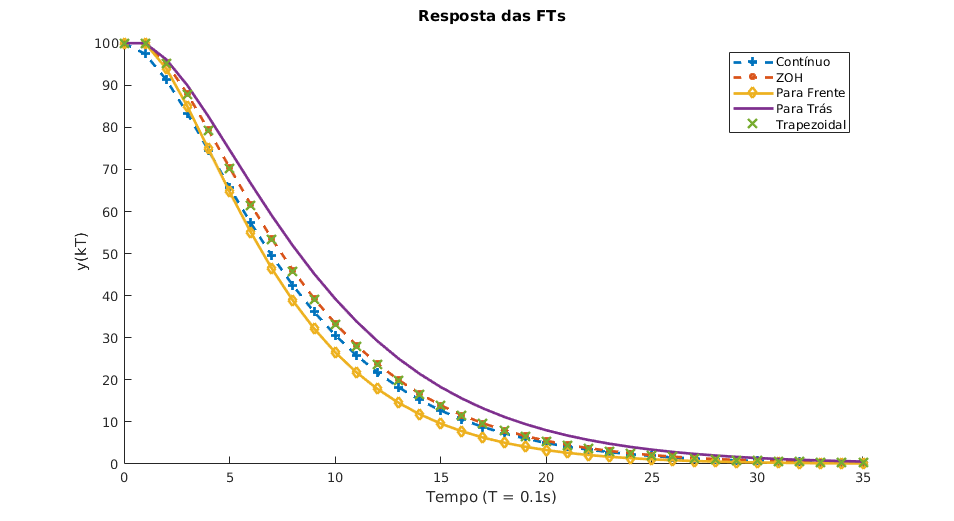
\includegraphics[width=1\linewidth]{images/discretizado.png}
            \caption{Gráfico de G(s) discretizado}\label{fig:discretizado}
    \end{figure}



%\section{Considere uma planta com entrada $u(t)$ e saída $y(t)$, cuja função de transferência é dada por $$ G(s) = \frac{Y(s)}{U(s)} = \frac{k_p}{Js^2} $$}
%\subsection*{Deseja-se utilizar um controlador com a estrutura $$ U(s) = \frac{bk_C}{a}U_c(s) - k_C\frac{s+b}{s+a}Y(s), $$ onde $U_C(s)$ é o sinal de referência. O polinômio característico de malha fechada deve ser $$ P(s) = (s+\omega_0)(s^2 + \omega_0s + \omega_0^2) = s^3 + 2\omega_0s^2 + 2\omega_0^2s + \omega_0^3. $$}
%\subsection*{Para isso, basta escolher os parâmetros do controlador como $a = 2\omega_0$, $b = \omega_0/2$ e $k_C = 2\frac{J\omega_0^2}{k_P}$. Nesse caso, é possível verificar que o tempo de acomodação de 5\% do sistema a malha fechada para a entrada degrau é $t_s(5\%) = 5.52/\omega_0$. Quando necessário, utilize $\omega_0 = 1$.}

%\subsection{Mostre que a função de transferência de malha fechada é dada por $$ \frac{Y(s)}{U_C(s)} = \frac{ (\frac{\omega_0^2}{2})\left( s + 2\omega_0\right) }{ s^3 + 2\omega_0s^2 + 2\omega_0^2s + \omega_0^3 }: $$}

    %\[ \frac{Y(s)}{U(s)} = \frac{k_P}{Js^2} \implies U(s) = \frac{Js^2}{k_P}Y(s) \]
    %\[ U(s) = \frac{Js^2}{k_P}Y(s) = \frac{bk_C}{a}U_c(s) - k_C\frac{s+b}{s+a}Y(s) \implies \left( \frac{Js^2}{k_P} + k_C\frac{s+b}{s+a} \right)Y(s) = \frac{bk_C}{a}U_c(s) \]
    %\[ \frac{Y(s)}{U_C(s)} = \frac{\frac{bk_C}{a}}{\frac{Js^2}{k_P} + k_C\frac{s+b}{s+a}} = \frac{ \frac{\omega_0/2}{2\omega_0} \frac{2J\omega_0^2}{k_P} }{ \frac{Js^2}{k_P} + \frac{2J\omega_0^2}{k_P} \left( \frac{s + \omega_0/2}{s + 2\omega_0} \right) } \]
    %\[ \frac{Y(s)}{U_C(s)} = \frac{\left( \frac{\omega_0^2}{2} \right)}{s^2 + 2\omega_0^2\left( \frac{s+\omega_0/2}{s+2\omega_0} \right)} = \frac{\left( \frac{\omega_0^2}{2} \right)(s+2\omega_0)}{s^2(s+2\omega_0) + 2\omega_0^2( s+\omega_0/2 )} = \frac{ (\frac{\omega_0^2}{2})\left( s + 2\omega_0\right) }{ s^3 + 2\omega_0s^2 + 2\omega_0^2s + \omega_0^3 } \]


%\subsection{Obtenha o diagrama de Bode do sistema a malha fechada e determine a frequência de corte $\omega_c$:}

    %%{O script para a geração do diagrama de Bode foi alterado a fim de encontrar a frequência de corte:}
%\begin{lstlisting}
%% https://www.mathworks.com/matlabcentral/answers/314007-bode-plot-and-cutoff-frequency
%clear
%close all

%global newx a b kc T

%J = 1;
%kp = 1;
%w0 = 1;
%a = 2*w0;
%b = w0/2;
%kc = 2*J*w0^2/kp;

%syscl = tf([w0^2/2 w0^3],[1 2*w0 2*w0^2 w0^3]);

%[mag,phase,wout] = bode(syscl);
%mag = squeeze(mag);
%phase= squeeze(phase);
%magr2 = (mag/max(mag)).^2;
%dB3 = interp1(magr2, [wout phase mag], 0.5, 'spline');
%figure(1)
%subplot(2,1,1)
%semilogx(wout, 20*log10(mag), '-b',  dB3(1), 20*log10(dB3(3)), '+r', 'MarkerSize',10)
%grid
%subplot(2,1,2)
%semilogx(wout, phase, '-b',  dB3(1), dB3(2), '+r', 'MarkerSize',10)
%grid
%\end{lstlisting}

    %\begin{figure}[H]
        %\centering
            %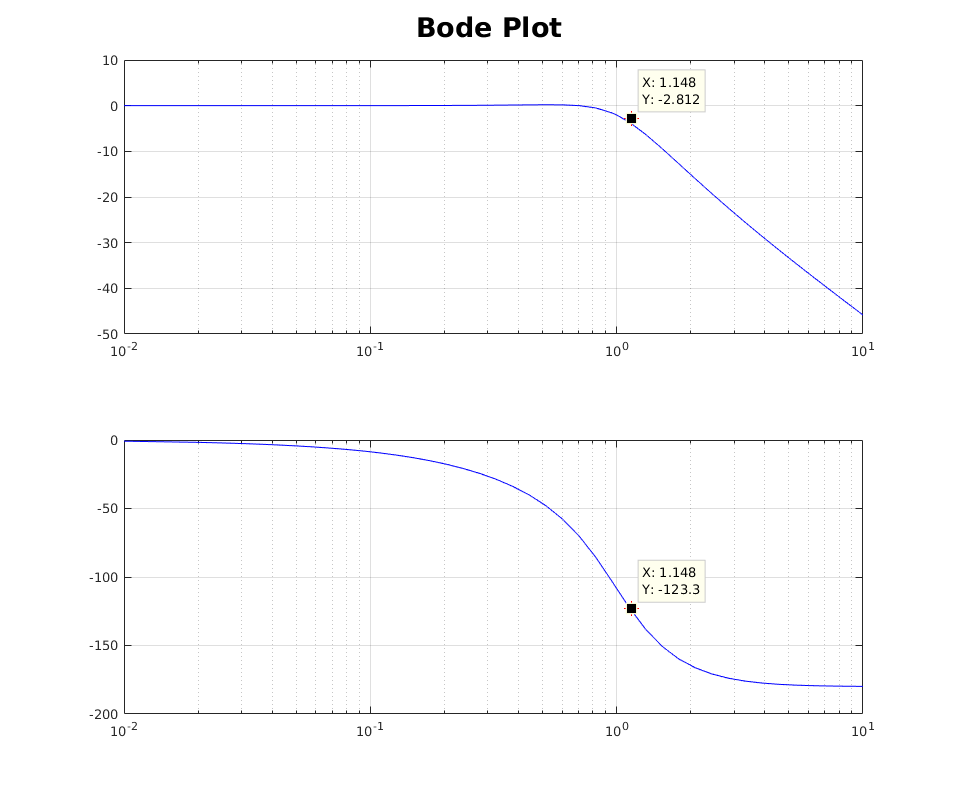
\includegraphics[width=1\linewidth]{images/bode_plot.png}
            %\caption{Diagrama de Bode}\label{fig:bode_plot}
    %\end{figure}

    %{Assim, temos a frequência de corte $\omega_c \approx 1.148$.}


%\subsection{Verifique que a ação de controle pode ser escrita como $$ U(s) = k_C \left( \frac b a U_C(s) - Y(s) + X(s) \right); $$ $$ X(s) = \frac{a-b}{s+a} Y(s). $$ Passando essas equações para o domínio do tempo e fazendo $\frac{dx(t)}{dt} \approx \frac{x(t+T)-x(t)}{T}$, onde $T$ é o período de amostragem, mostre que o controlador pode ser discretizado da seguinte forma $$ u[k] = k_C \left( \frac b a u_c[k] - y[k] + x[k] \right); $$ $$ x[k+1] = x[k] + T\left[ (a-b)y[k] - ax[k]\right] : $$}
    %\[ U(s) = \frac{bk_C}{a}U_c(s) - k_C\frac{s+b}{s+a}Y(s) = k_C\left( \frac b a U_C(s) - \frac{s+b}{s+a}Y(s) \right) = k_C\left( \frac b a U_C(s) + \left( \frac{-s-b}{s+a} \right) Y(s) \right)  \]
    %\[ U(s) = k_C\left( \frac b a U_C(s) + \left( \frac{-s-b+a-a}{s+a} \right) Y(s) \right) = k_C\left( \frac b a U_C(s) + \left( \frac{-s-a}{s+a} + \frac{a-b}{s+a} \right) Y(s) \right) \]
    %\[ U(s) = k_C\left( \frac b a U_C(s) -Y(s) + \left( \frac{a-b}{s+a} \right) Y(s) \right) = k_C \left( \frac b a U_C(s) - Y(s) + X(s) \right) \]
    %\[ u[k] = k_C\left( \frac b a u_C[k] - y[k] + x[k] \right) \]
    %\[ \frac{dx(t)}{dt} \approx \frac{x(t+T) - x(t)}{T} \implies \frac{x[k+1]-x[k]}{T} \approx \frac{dx(t)}{dt} \]
    %\[ x(s) = \frac{a-b}{s+a}y(s) = (a-b)y(s)\frac{1}{s+a} \implies \frac{dx(t)}{dt} = (a-b)y[k] - ax[k] \implies \frac{x[k+1]-x[k]}{T} \approx (a-b)y[k] - ax[k] \]
    %\[ x[k+1] = x[k] + T((a-b)y[k] - ax[k])\]


%\subsection{Implemente no Simulink esse sistema com controlador a tempo contínuo e com controlador discretizado com períodos de amostragem $T = 0.2/\omega_0$, $T = 0.5/\omega_0$ e $T = 1.08/\omega_0$:}
    %\begin{figure}[H]
        %\centering
            %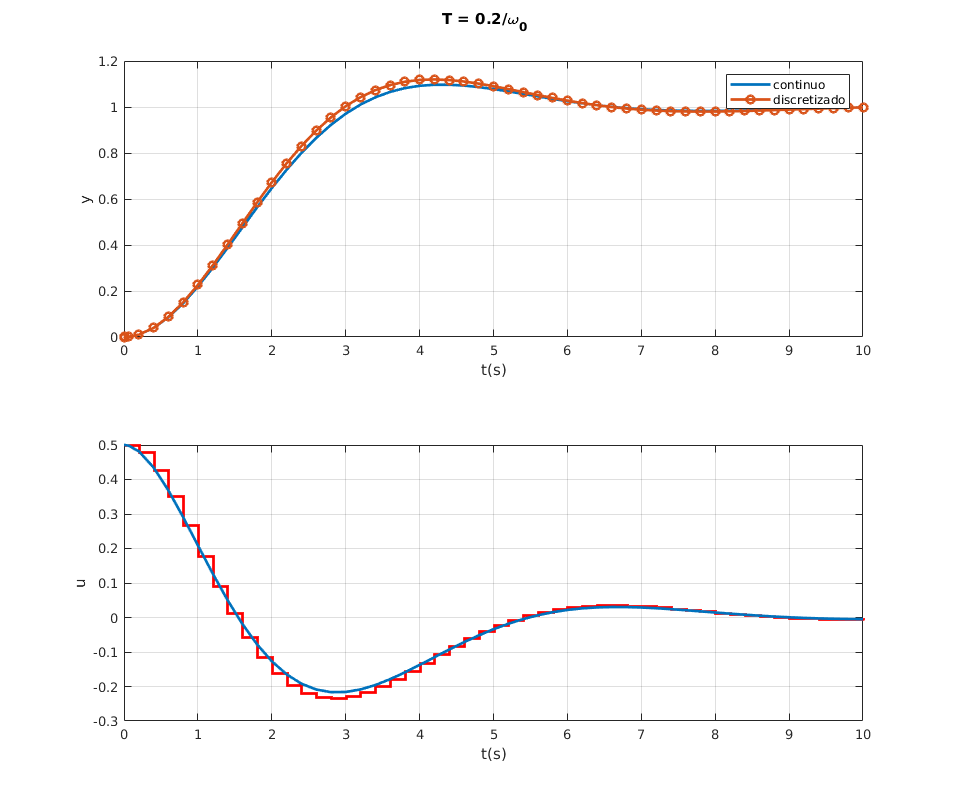
\includegraphics[width=.7\linewidth]{images/periodo_02.png}
            %\caption{Resposta e sinal de controle para período $T = 0.2\omega_0$.}\label{fig:periodo_02}
    %\end{figure}

    %\begin{figure}[H]
        %\centering
            %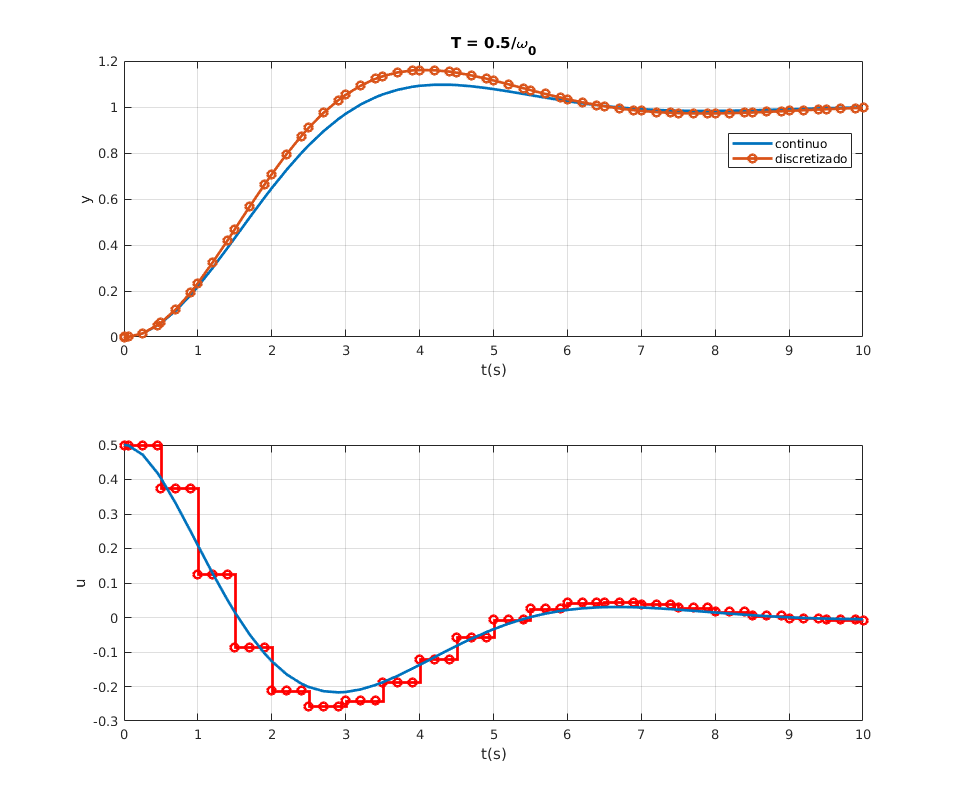
\includegraphics[width=.7\linewidth]{images/periodo_05.png}
            %\caption{Resposta e sinal de controle para período $T = 0.5\omega_0$.}\label{fig:periodo_05}
    %\end{figure}

    %\begin{figure}[H]
        %\centering
            %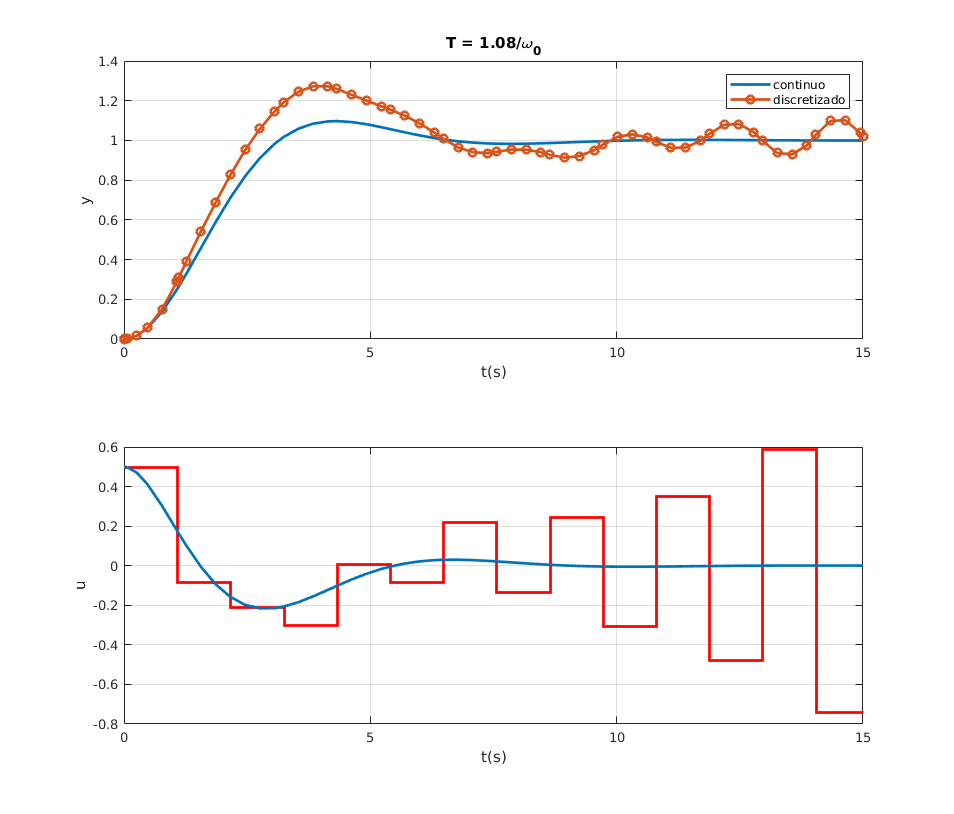
\includegraphics[width=.7\linewidth]{images/periodo_108.png}
            %\caption{Resposta e sinal de controle para período $T = 1.08\omega_0$.}\label{fig:periodo_108}
    %\end{figure}


%\subsection{Para cada período de amostragem, calcule a relação entre a frequência de amostragem e a frequência de corte do sistema a malha fechada $\omega_s/\omega_c$:}
    %\[ \textrm{Para } T = 0.2/\omega_0  \implies \frac{\omega_s}{\omega_c} \approx 4.355 \]
    %\[ \textrm{Para } T = 0.5/\omega_0  \implies \frac{\omega_s}{\omega_c} \approx 1.742 \]
    %\[ \textrm{Para } T = 1.08/\omega_0 \implies \frac{\omega_s}{\omega_c} \approx 0.968 \]


%\subsection{Para cada período de amostragem, compare a saída do sistema a malha fechada com controlador contínuo com a saída do sistema a malha fechada com controlador discretizado. O que se pode afirmar sobre o tempo de assentamento para os sistemas com controlador discretizado?}
    %{De acordo com a simulação, quanto menor o período de amostragem, menor o
    %tempo de assentamento para o sistema dado. Caso o período de amostragem seja
    %grande, o sistema se torna instável, como observado para $T = 1.08/\omega_0$.}


%\subsection{Para cada período de amostragem, compare a ação de controle do sistema em malha fechada com controlador contínuo com a saída do sistema em malha fechada com controlador discretizado:}
    %{Para $T = 0.2/\omega_0$, a resposta do sistema discreto em malha fechada foi
    %extremamente próxima da resposta a tempo contínuo.}

    %{Para $T = 0.5/\omega_0$, a resposta do sistema discreto em malha fechada teve
    %um \textit{overshoot} levemente maior que o da resposta a tempo contínuo.}

    %{Para $T = 1.08/\omega_0$, a resposta do sistema discreto em malha fechada é instável.}


%\subsection{O que pode ser concluído acerca da seleção da frequência de amostragem para a discretização de controladores a tempo contínuo?}
    %{Nessa simulação, frequêcias de amostragem mais altas representaram uma
    %resposta do sistema a tempo discreto mais próximas da resposta a tempo
    %contínuo, e frequências mais baixas tenderam à instabilidade do sistema.}


\end{document}

